Most real world networks are incomplete \cite{kim2011network, wang2014link}. These networks lie somewhere in the range of a deterministic and a purely random structure, and are thus partially predictable \cite{lu2015toward}. Link prediction is the problem of identifying potentially missing/undiscovered connections in such networks \cite{marchette2008predicting, kim2011network}, or even forecasting future connections \cite{bringmann2010learning, juszczyszyn2011link}, by examining the current network structure\ignore{\cite{zhou2021progresses}}. This is useful in various applications, such as recommending items for online purchase \cite{akcora2011network}, helping people to find potential collaborators \cite{mori2012machine, tang2012cross},\ignore{predicting co-authorships in academic research networks \cite{pavlov2007finding, wohlfarth2008semantic}, identifying abnormal communications \cite{huang2009time}} assessing trustworthiness of individuals \cite{alnumay2019trust}, uncovering criminal activities and individuals \cite{berlusconi2016link, lim2019hidden}\ignore{, detecting anomalies \cite{huang2006link}}, and predicting new protein-protein interactions or generating hypotheses \cite{cannistraci2013link, nasiri2021novel}.

Similarity measures are frequently employed to predict the likelihood of missing or future links between unconnected nodes in a network \cite{wang2014link, arrar2023comprehensive}. The principle is straightforward: higher similarity indicates a greater likelihood of connection \cite{wang2014link}. The choice of metric depends on the network's characteristics, with no single metric dominating across different datasets \cite{arrar2023comprehensive, zhou2021progresses}. Local / neighborhood-based similarity metrics such as Common Neighbors\ignore{\cite{newman2001clustering}}, Jaccard Coefficient\ignore{\cite{jaccard1901etude}}, S{\o}rensen Index\ignore{\cite{sorensen1948method}}, Salton Cosine similarity\ignore{\cite{salton1973specification}}, Hub Promoted\ignore{ \cite{liben2003link}}, Hub Depressed, Leicht-Holme-Nerman, Adamic-Adar\ignore{\cite{adamic2003friends}}, and Resource Allocation\ignore{\cite{zhou2010solving}}, which are based of are based on neighborhood information within a path distance of two, remain popular \cite{arrar2023comprehensive, wang2014link}. This is due to their simplicity, interpretability \cite{pai2019netdx, barbieri2014follow}, computational efficiency \cite{garcia2014link}, and the ability to capture underlying structural patterns.\ignore{Further, they are often combined with other metrics.}

However, many studies \cite{gatadi2023lpcd, saifi2023fast, benhidour2022approach, mumin2022efficient, rafiee2020cndp, guo2019node, yang2015new, papadimitriou2012fast, wang2019link} and network analysis software \cite{staudt2016networkit, csardi2006igraph} use a baseline approach for link prediction, computing unnecessary similarity scores for all non-connected node pairs. Further, early studies often evaluate a limited number of algorithms on small networks --- this can result in misleading conclusions \cite{zhou2021progresses, zhou2021experimental}. Further, much existing research does not address link prediction for large networks with close to a billion edges \cite{muscoloni2022adaptive, mumin2022efficient, nasiri2021novel, xian2021towards, ghasemian2020stacking, mara2020benchmarking, wang2019link, xu2019distributed, mohan2017scalable, cui2016bounded, garcia2014link, papadimitriou2012fast}. As the collection of data, represented as graphs, reach unprecedented levels, it becomes necessary to design efficient parallel algorithms for link prediction on such graphs. While link prediction algorithms are often pleasingly parallel, most studies do not address the design of suitable data structures for efficient computation of scores.

Further, the link prediction problem faces significant imbalance, with the number of known present links often several order of magnitude less than known absent links. This imbalance hinders the effectiveness of many link prediction methods, particularly on large networks \cite{wang2014link, garcia2014link}. Thus, heuristics are needed to minimize the computation needed, without sacrificing on quality.\ignore{To assess the accuracy of link prediction algorithms, observed links $E$ are split into a training set $E^T$ and a probe set $E^P$ for evaluation.} Quality assessment measures for link prediction include precision, recall, F1 score, accuracy, and Area Under the Receiver Curve (AUC). While AUC is commonly used \cite{arrar2023comprehensive}, it may provide misleading results\ignore{, by giving high scores to algorithms that successfully rank many negatives in the bottom} \cite{yang2015evaluating, lichtnwalter2012link}, leading to our focus on F1 score.

\ignore{How do you explore the neighbors of each node, and compute intersection? What is a super naive way to do the above?}




\subsection{Our Contributions}

In this report, we introduced two novel approaches, namely IHub and LHub, for efficient link prediction in large graphs. The IHub approach is an enhanced parallel method that efficiently finds common neighbors and handles large graphs by tracking top-$k$ edges per-thread and later merging them globally. LHub is a heuristic approach which additionally discards large hubs, based on the observation that low-degree nodes contribute significant similarity among neighbors. We then experimentally determined suitable hub limits, i.e, the degree above which a vertex is considered as a large hub, for link prediction with each similarity metric.

On a machine with two 16-core Intel Xeon Gold 6226R processors, our results show that the LHub approach outperforms IHub by over $963\times$ and $163\times$ on average with $10^{-2}|E|$ and $0.1|E|$ unobserved edges, respectively. This speedup is achieved while maintaining comparable F1 scores. Notably, LHub achieves a link prediction rate of $38.1M$ edges/s with $0.1|E|$ unobserved edges. We also identified suitable similarity metric for each type of graph. When predicting $0.1|E|$ edges with the LHub approach, we observed that $63\%$ of the runtime is spent on the scoring phase, and especially higher on social networks, with high average degree. With doubling of threads, LHub exhibits an average performance scaling of $1.7\times$.




%% - Use --- for a dash.
%% - Use ``camera-ready'' for quotes.
%% - Use {\itshape very} or \textit{very} for italicized text.
%% - Use \verb|acmart| or {\verb|acmart|} for mono-spaced text.
%% - Use \url{https://capitalizemytitle.com/} for URLs.
%% - Use {\bfseries Do not modify this document.} for important boldface details.
%% - Use \ref{fig:name} for referencing.

%% For a block of pre-formatted text: 
% \begin{verbatim}
%   \renewcommand{\shortauthors}{McCartney, et al.}
% \end{verbatim}

%% For a list of items:
% \begin{itemize}
% \item the ``ACM Reference Format'' text on the first page.
% \item the ``rights management'' text on the first page.
% \item the conference information in the page header(s).
% \end{itemize}

%% For a table:
% \begin{table}
%   \caption{Frequency of Special Characters}
%   \label{tab:freq}
%   \begin{tabular}{ccl}
%     \toprule
%     Non-English or Math&Frequency&Comments\\
%     \midrule
%     \O & 1 in 1,000& For Swedish names\\
%     $\pi$ & 1 in 5& Common in math\\
%     \$ & 4 in 5 & Used in business\\
%     $\Psi^2_1$ & 1 in 40,000& Unexplained usage\\
%   \bottomrule
% \end{tabular}
% \end{table}

%% For a full-width table:
% \begin{table*}
%   \caption{Some Typical Commands}
%   \label{tab:commands}
%   \begin{tabular}{ccl}
%     \toprule
%     Command &A Number & Comments\\
%     \midrule
%     \texttt{{\char'134}author} & 100& Author \\
%     \texttt{{\char'134}table}& 300 & For tables\\
%     \texttt{{\char'134}table*}& 400& For wider tables\\
%     \bottomrule
%   \end{tabular}
% \end{table*}


%% For inline math:
% \begin{math}
%   \lim_{n\rightarrow \infty}x=0
% \end{math},

%% For a numbered equation:
% \begin{equation}
%   \lim_{n\rightarrow \infty}x=0
% \end{equation}

%% For an unnumbered equation:
% \begin{displaymath}
%   \sum_{i=0}^{\infty} x + 1
% \end{displaymath}

%% For a figure:
% \begin{figure}[h]
%   \centering
%   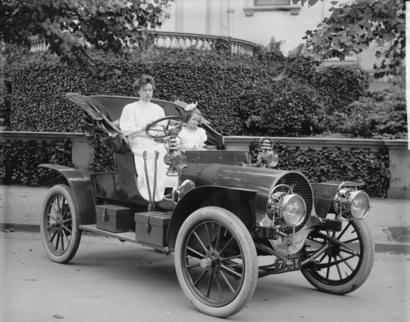
\includegraphics[width=\linewidth]{inc/sample-franklin}
%   \caption{1907 Franklin Model D roadster. Photograph by Harris \&
%     Ewing, Inc. [Public domain], via Wikimedia
%     Commons. (\url{https://goo.gl/VLCRBB}).}
%   \Description{A woman and a girl in white dresses sit in an open car.}
% \end{figure}

%% For a teaser figure.
% \begin{teaserfigure}
%   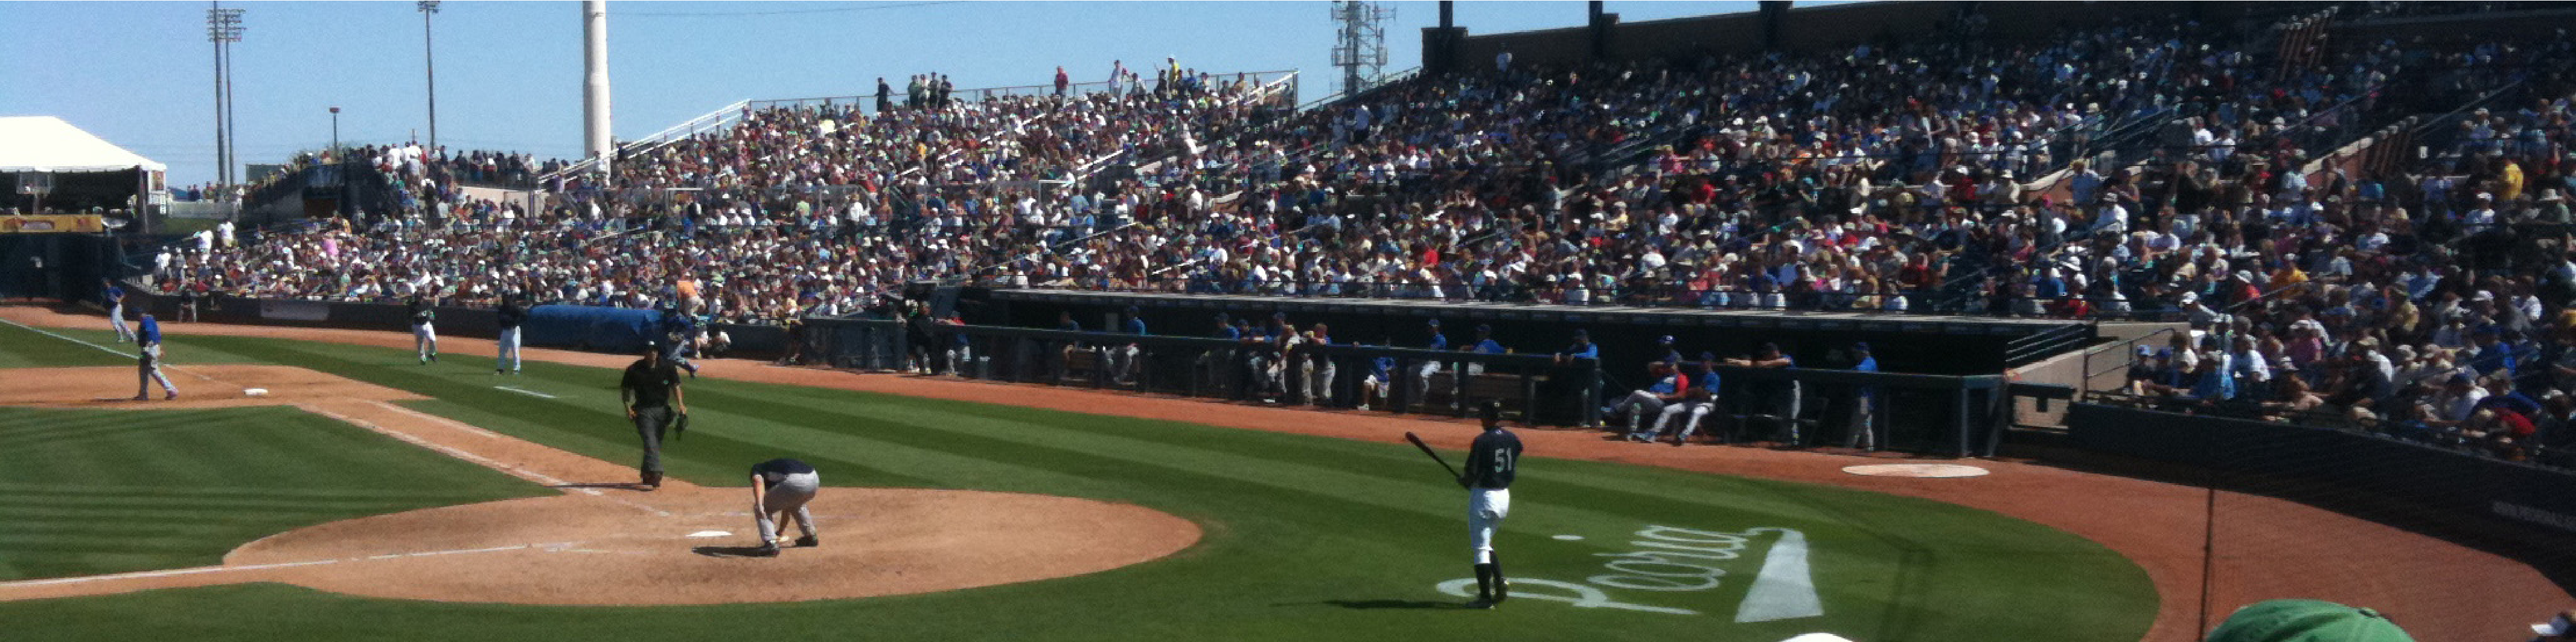
\includegraphics[width=\textwidth]{sampleteaser}
%   \caption{figure caption}
%   \Description{figure description}
% \end{teaserfigure}
